\documentclass[./../main.tex]{subfiles}
\graphicspath{{img/}}
\begin{document}
	\begin{exercise}
		Determina el momento de inercia del núcleo de \ch{^{170}Hf} de acuerdo a la \cref{fig:hafmio-rot-spectrum}, un valor por cada energía y \(J^{\pi}\) o si deseas puedes hacer una gráfica \(J^{\pi}\) vs. \(E\).

		\begin{figure}[htb]
			\centering
			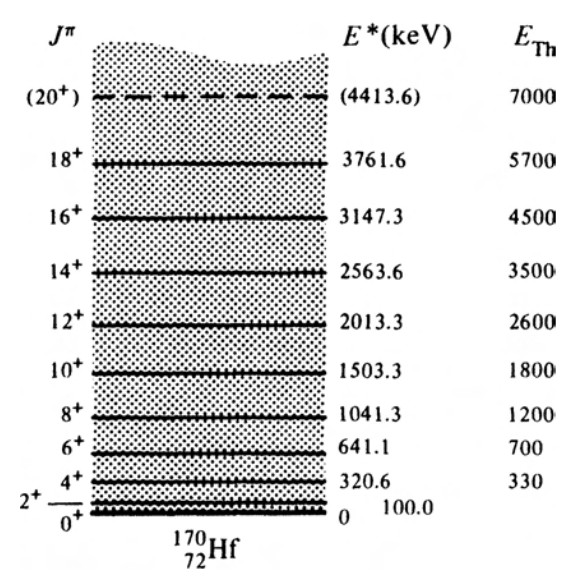
\includegraphics[scale=0.4]{rot_spectrum}
			\caption{Espectro rotacional del núcleo deformado \ch{^{170}Hf}.}			
			\label{fig:hafmio-rot-spectrum}
		\end{figure}
	\end{exercise}
\end{document}
